% !TeX root = ../../main.tex
% Add the above to each chapter to make compiling the PDF easier in some editors.

\section{Interactive Segmentation}\label{ord:ch2:sec3}

Image segmentation takes as input $x$ only the image itself, in contrast interactive segmentation takes beside the image some additional information interactively provided by an user as input.
% Interactive segmentation segmentation takes advantage of additional information interactively provided by an user.
This additional information is especially beneficial, because it is manually picked by the valuable image processing capabilities of human users.
Due to this, interactive segmentation networks are provided with high level guidance regarding the objects location.
Depending on the type of interaction, the receipt of the user input may be more or less elaborately, which leads to a fundamental difficulty of interactive methods in general.
User interaction may be considered expensive and elaborate.
% Especially, for deep learning tasks a great quantity of images is required.

% TODO interactive segmentation methods on semantic segmentaiton?
Instance segmentation is a common task for the application of interactive methods.
%, but may also be used for semantic segmentation is applicable in the given context.
They focus on extracting one object from an image, so the prediction basically distinguish between two classes: the foreground object to segment and the background.
In order to segment multiple objects in an image or the whole image, usually multiple iterations are necessary.
% TODO scope of interactive segmentation here, the class is assigned manually?
In the following the principles of several concepts for interactive segmentation methods are introduced.

\subsection{Classical Concepts}\label{ord:ch2:sec3:subsec1}
Before the upcomming of \gls{dl} and \glspl{cnn}, segmentation was already performed with classical image processing.
These methods also focus on the extraction of a foreground object from the background by little user interaction.

% GraphCut and GrabCut
Prominent algorithms are Graph Cut \cite{BJ01-GraphCut} and GrabCut \cite{RKB04-GrabCut}.
As user interaction GrabCut requires a loose bounding box.
Everything outside the bounding box and the borders itself are defined as background, while the inside of the box is segmented based on contrast and color information.
Further, the goodness of the result may be enhanced by iteratively defining explicit image parts as fore- or background.

% Watershed
Another still relevant method to perform instance segmentation is the Watershed algorithm \cite{NS94-Watershed}.
This method interactively collects fore- and background regions from an user in order to perform segmentation.
The Watershed algorithm is part of the benchmark study and elaborately examined in Chapter \ref{ord:ch3}.

% Superpixels
Last, an algorithm using so-called \textit{Superpixel} was introduced in 2003 \cite{RM03-Superpixel}.
Superpixels are groups of connected pixels, that share similarities in color or low-level features as contour, brightness or texture.
Further, these Superpixels are used to perform segmentation.
This algorithms is still a current research topic, an overview of several state-of-the-ar approaches is given in \cite{SHL16-SuperpixelEvaluation}.
 
% Final tought
These classical methods may perform very well on certain images, but tend to reach their limitations as they deal with more complex structures.
They are often outperformed on current benchmark datasets by more recent \gls{dl} methods.
% This is due to their rather simple processing of superficial characteristics \eg edges, textures, contrast and color.
% On the contrary \gls{dl} based methods are capable to examine images on a deeper level and so understand more complicated structures.


\subsection{\gls{dl} User Point Concepts}\label{ord:ch2:sec3:subsec2}

\subsubsection{Basic Concept}
% DL focus 
Mordern interactive segmentation algorithms combine \gls{dl} models and additional user input.
As \gls{dl} models usually \glspl{cnn} for image segmentation are applied.
% Obtaining points on fore- and background
User point centered concepts obtain the user input in the form of clicks on the image.
The user clicks are often differentiated between clicks on the foreground object and clicks on the background.
The input $x$ of an interactive segmentation network is a combination of the image and the user clicks.

% TODO probability map
This fundamental concept is used for various interactive segmentation models \cite{Xu16-InteractiveObjectSelection} \cite{MVL18-ITIS} and exemplary shown in Figure \ref{fig:ch2:sec3:ifcn}
% IOG and DEXTR explained in detail in following chapter.
Further, the methods \gls{dextr}  \cite{Man18-DEXTR} and \gls{iog} \cite{Zha20-IOG} also follow a user point centered concept. They are part of the benchmark and extensively described in Chapter \ref{ord:ch3}.
\begin{figure}
	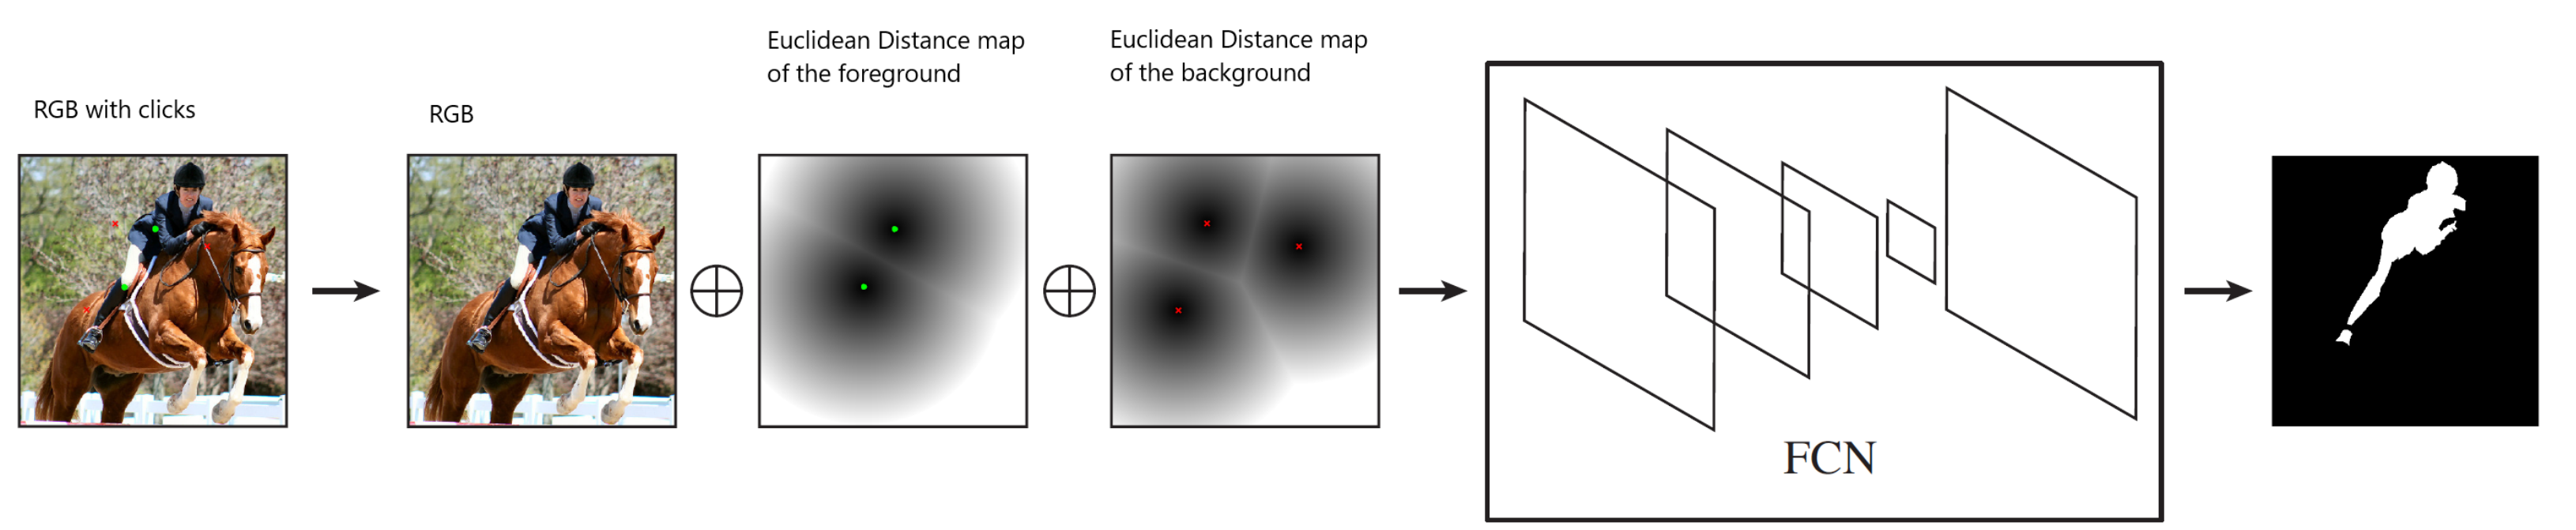
\includegraphics[width=\linewidth]{figures/chap232_ifcn.png}
	\caption[Interactively Fully Convolutional Network]{ Copyright \copyright 2016 IEEE. Reprinted by permission from \cite{Xu16-InteractiveObjectSelection}}
	\label{fig:ch2:sec3:ifcn}
\end{figure}

\subsubsection{Representation of User Clicks and Model Input}
The user clicks are converted to points and mapped into new heatmaps, that have the same spacial dimension as the input image.
In order to distinguish between fore- and background points, there exist separate heatmaps for fore- and background.
In some literature the foreground points are also called \textit{positive} points, while the background points are called \textit{negative} points.
If there is are only one type of points, there also exist only one heatmap.

% Modification of points -> gauss or euclidean
The heatmaps are further processed, in order to highlight the set user points.
This may be achieved by the conversion into an Euclidean distance map \cite{Dan80-EuclideanDistanceMapping} or the application of a Gauss filter.
% TODO source or footnote for Gauss filter

% 3 RGB Channels + 2 Heatmaps = 5-Channel input
The image usually is a colored RGB image of three channels.
The heatmaps have the same size as the image and are appended to the image as additional channels.
%This results in a five- or four-channel input for the interactive segmentation network, depending on the number of heatmaps.
This results in a five-channel input using fore-and background heatmaps or in a four-channel input using just a foreground heatmap.
So the processed points on the heatmaps and the user clicks on the image are located exactly at the same position on different channels.
This matching is vital for the segmentation network, in order to locate and differentiate fore- and background.
The multidimensional input functions as model input $x$ for the semantic segmentation network.

Interactive segmentation networks are often based on normal segmentation networks, \eg the \gls{fcn} in the \gls{ifcn} \cite{Xu16-InteractiveObjectSelection} or the DeepLabv3+ in the \gls{itis} network \cite{MVL18-ITIS}.
As for segmentation networks, the prediction $\hat{y}$ of interactive networks is a probability map.

\subsubsection{Interactive Refinement}
A fundamental advantage of interactive methods is the presence of a human user.
The interactive segmentation network may not always deliver a satisfactory result in the initial execution.
For this case, interactive methods often provide the option to refine the initial result.
In order to apply refinement, the user often sets an additional click on the fore- or background region, where the segmentation fails.
This refinement click is added to the corresponding heatmap and therefore included in the multidimensional input.
After obtaining the updated input, the network requires another execution.
This refinement process may be applied iteratively by the user.

With refinement the guidance provided by the user is additionally reinforced.
Further, interactive refinement specifically focuses on regions of failure, while other models without user interaction must rely on their initial predictions.



\subsubsection{Characteristics}
% Similar to normal segmentation networks.
Interactive segmentation networks almost have the same characteristics as normal segmentation networks.
For training they require the multidimensional input $x$, while the label $y$ remains the same.
% Simulation of user clicks.
In order to simplify training and evaluation, user clicks are regularly simulated.
The simulation of the user clicks is based on the corresponding \gls{gt}.
To apply a simulation has certain advantages compared to manually acquiring user clicks.
First, simulations are easily scalable, faster and cheaper than the acquisition of manual clicks from real users.
Second, in a simulation no variance occurs between the set clicks of various users, if the .
% TODO is this necesarrily an advantag?
Third, simulations have the possibility to effortless create various click patterns, that \eg vary the set click by a random offset, in order to simulate a various types of user behavior.

% Refinement Training
The training setup for iterative refinement is more elaborate.
The refinement clicks are simulated online during the training process.
In the simulation the refinement clicks are usually set on the greatest error, which is calculated based on the \gls{gt} and the prediction $\hat{y}$ of the previous model execution.

\subsubsection{Variations}
% Special Methods 
%    - Iterative learning
%    - Fusion networks
While the presented concepts is the most common approach and achieves state-of-the-art results, there are other mention-able ideas and variations:
\begin{itemize}
	% One click
	\item \textbf{One-Click Segmentation} is introduced in \cite{Maj20-One-Click} and this networks requires only one click one foreground click.
	This click is processed as foreground click and enforced with a Gauss filter.
	The segmentation is based on the DeepLab network.
	Despite the user interaction is most simple, this approach can not compete with the performance of state-of-the-art networks.
	
	\item The \textbf{\gls{fctsfn}} stands out, due to the separate processing of image and user clicks \cite{Hu19-TwoStreamFusionNetwork}.
	% The fore- and background points are converted into two feature maps, that contain an Euclidean distance map.
	The user clicks and the image are processed separately by two streams.
	These two processing streams share the same architecture based on VGG16, but have their own weights.
	The intent is to learn the deep features from image and user clicks individually.
	Further, the two streams are combined and processed together to create one prediction.
	
	\item \textbf{Iterative training} is applied in the \gls{itis} network \cite{MVL18-ITIS}.
	Every epoch a new refinement click is added to the multidimensional input.
	This click is simulated during the training process, based on the classification result of the previous epoch.
	It is claimed, that this novel \textit{iterative training procedure} significantly improves the networks performance.
	
\end{itemize}


\subsubsection{Evaluation and State-of-the-Art Networks}
% Describe Evaluation metrics: clicks requried for certain iou and iou at certain amount of clicks
For a reliable evaluation of interactive methods the user interaction has to be taken into account.
For user interactions based on clicks, two metrics are widely used together, represented in Table \ref{tab:ch2:interactive-stae-of-the-art}. 
The first metric lists the number or clicks, that a model requires to reach a certain level of performance. 
The number of clicks must not be even, due to the averaging of all results of the dataset.
The second metric lists the models performance for a certain amount of clicks.

% Limitations.
Yet, with these metrics, a uniform evaluation reaches some limitations, addressed in the following:
The first metric is actually only applicable if a method has the possibility to perform refinement.
The second metric does not always enable a fair comparison, because for various methods the underlying functioning may be different. 
For example, the minimal required amount of clicks may be lower or higher than the amount of clicks, which is set for comparison.

% Problems with the evaluation of time.
In terms of interactive methods, the time required for the user interaction is fundamental for the evaluation.
The measured time by single papers is not comparable, due to the missing of a common setup to perform uniform user studies for these novel methods.
With these metrics the time is only approximated by the number of clicks.
But there are no indicators, that describes how elaborate it is and how much time it needs to set these clicks.
Further, there is no common metric to evaluate the usability of these interactive methods

Nevertheless, these metrics are the current state to evaluate interactive segmentation methods.
They are still suitable to meaningful compare interactive segmentation models, but their limitations have to be noted.
A comparison of several mentioned methods and the current state-of-the-art methods is given in Table \ref{tab:ch2:interactive-stae-of-the-art}.


% State of the art
\begin{table}[h!]
	\centering
	\begin{tabular}{l|c|c}
		\textbf{Model} & \textbf{Number of clicks} & \textbf{\gls{iou} (\%) @ 4 clicks} \\
		& Pascal VOC @85\% & Pascal VOC \\
		\hline
		% TODO add watersheds if available for PASCAL VOC
		Graph Cut \cite{BJ01-GraphCut}									  & > 20 & 41.1\\
		\glsentryshort{ifcn} \cite{Xu16-InteractiveObjectSelection}       & 6.9  & 75.2\\
		\glsentryshort{risnet} \cite{Liew17-RegionalInteractiveImageSeg}  & 5.7  & 80.7\\
		\glsentryshort{itis} \cite{MVL18-ITIS}			 				  & 3.4  & -\\
		\glsentryshort{fctsfn} \cite{Hu19-TwoStreamFusionNetwork}		  & 4.6  & -\\
	    \glsentryshort{dextr} \cite{Man18-DEXTR} 	     				  & 4    & 91.5\\
		\glsentryshort{iog} \cite{Zha20-IOG}	 	    				  & 3    & 94.4\\
	\end{tabular}
	\caption[Comparison of interactive segmentation models.]{
		Comparison of interactive segmentation models on the Pascal VOC 2012 test set.
		It can be seen, that interactive segmentation methods have developed quickly. 
		They strongly improved in terms of required clicks and \gls{iou}.
		% TODO ?? Pascal VOC is at its limit to be suitable to evaluate semantic segmentation.
	}
	\label{tab:ch2:interactive-stae-of-the-art}
\end{table}

\subsection{\gls{dl} Polygon Concepts}\label{ord:ch2:sec3:subsec3}
This concept is based on the idea to use a \gls{dl} model to predict a polygon.
The polygon represents the segmentation mask and within the desired object.

The following is a brief summary of the method represented in \cite{Ling19-Curve-GCN}.
% Workflow + UI
As initial user interaction a loose bounding box around the object of interest is required.
Based on this box the image is cropped and the crop is used as model input.

% Architecture
The \gls{dl} model consists out of a combination of several subnetworks and architectural components.
First, a \gls{cnn} takes the cropped image as input and performs as encoder.
This encoder provides the extracted features and a boundary prediction to the third component.
Second, a fixed size polygon is initialized, to transform the task into a graph problem.
Third, a multi-layer \gls{gcn} iteratively shifts the position of each polygon node towards the object boundary.
This method is named \textit{Curve-\gls{gcn}}, inspired by the \textit{curved} approximation of a closed polygon.

% Good user interaction - refinement
The user is able to perform refinement, by interactively moving single nodes of the polygon.
% Performance
% The performance of the \textit{Curve-\gls{gcn}} is only represented on the Cityscapes Dataset, but it claim to perform 
Details of this method can be reviewed in \cite{Ling19-Curve-GCN}.

% Vorreiter von Curve GCN \cite{Acu18-Polygon-RNN++}
The predecessor of the \textit{Curve-\gls{gcn}} is based on \glspl{rnn} and introduced in \cite{Acu18-Polygon-RNN++}.





